%
% File: chap05.tex
% Author: Antigoni Kourou
% Description: Evaluation
%


\let\textcircled=\pgftextcircled
\chapter{Evaluation}
\label{chap:eva}
\initial{F}or checking the efficiency of the proposed pipeline, its performance is compared to human logic for two main purposes. First, the evaluation aims to find out how well VADER, the selected sentiment detection algorithm, performs in the chosen dataset and secondly, how well can the pipeline identify the features of a certain sentence of review. To answer these two questions, a sample of 100 text reviews are randomly chosen from the dataset and are given to humans for evaluation. Each respondent is required to first read the sentences, then to estimate a score of sentiment for each of them on a scale from -1 to +1 and finally to mark the accommodation features, which the sentence in question refers to. These tasks are similar to what the pipeline is programmed to do. 
% Evaluation form in Appendix 
The evaluation form is completed by 5 humans, who come from different educational backgrounds, are geographically diverse and are Airbnb users. Their answers are analyzed and compared to the pipeline output using SPSS. Considering the diversity between users and in order to understand the common human logic, their evaluations are firstly compared to each other using correlation values between samples and distribution statistics. This analysis showed that three of the respondents had very similar answers, consisting in a correlation varying between 72\% to 83 \% between each other and a very similar distribution curve. 
%These output of the analysis in SPSS can be found in Appendix. 
Based on these results, the chosen sample to represent the average human logic are the average rates of the three "unbiased" respondents. 

\section{Evaluation of VADER algorithm}
VADER is considered to be one of the best algorithms for sentiment mining with a very high accuracy \cite{hutto2014vader}. However, when VADER was tested to perform in 22 different datasets, it was noticed an overall accuracy of 78.7\%, which varies significantly from one dataset to the other \cite{ribeiro2015benchmark}. To clear all the doubts of how VADER would perform on reviews and specifically in the chosen dataset of this research, its scores are compared to the average human rating. The correlation between the two sets based on cases results to be 70.8\%. Although, this value is lower than the average case of VADER's accuracy, it indicates a satisfactory scale of accuracy for the Airbnb dataset. From Figure \ref{fig:distribution} can be noticed that the two datasets share the same mean (4.125 compared to 4.13) and have similar standard deviations. 
\begin{figure}[h!]
	\centering
	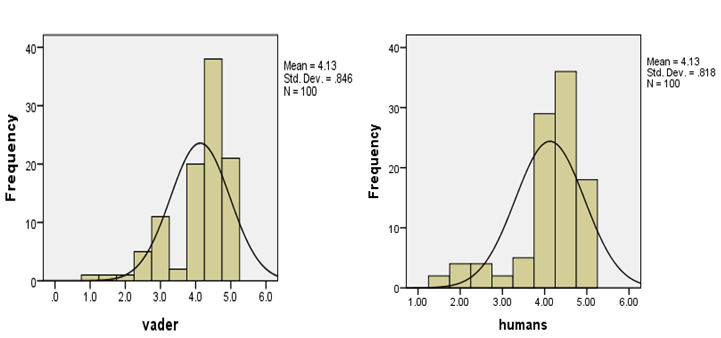
\includegraphics[height=0.33\textheight]{graphs_vader_humans}
	\caption{Distribution of VADER and humans' sentiment scores}
	\label{fig:distribution}
\end{figure}
The differences between VADER scores and human evaluation are also calculated and they result in 53\% of cases when VADER has detected the exact score as human logic, 24\% cases where the difference is just half a star, 14\% cases with one star difference and the 9\% cases with more than one star difference. The last ones form the group of "errors" in VADER sentiment scores. The highest value of error is 2.5 stars, in only 3\% cases, which means that VADER will never consider a very positive sentence as a very negative one and the other way round. However, it may consider these kind of sentences as neutrals or may be confused of the sign of sentences with slight sentiment.

\section{Evaluation of feature identification part}
The effectiveness of the proposed technique for feature identification is measured by using precision, recall and accuracy as suggested by \cite{huang2006performance}. The values are calculated for each of the features as:
$$ Precision  (p) =\frac{TP}{TP+FP}\hspace{1cm}(2)$$
$$ Recall  (r) = \frac{TP}{TP + FN}\hspace{1.6cm}(3) $$
$$ Accuracy (a) = \frac{TP + TN}{TP+TN+FP+FN} \hspace{1cm}(4)$$
where TP (true positives) is the number of sentences that the algorithm correctly identifies the right features; FP (false positives) is the number of sentences that the algorithm falsely extract wrong features; FN (false negatives) is the number of sentences that the algorithm fails to identify the right features and TN (true negative) is the number of sentences that the algorithm correctly does not identify any feature. The average human logic identifies a feature in a sentence when it is agreed by the majority of respondents. Ideally the algorithm shall have values of precision and recall close to 1 for each of the features. This evaluation of the pipeline as illustrated in Figure \ref{fig:matrix} shows that the algorithm manages to identify some features better than others. For example the \textit{value} and \textit{cleanliness} features of the listing are identified almost always with high precision and recall, but a low precision for \textit{communication} means that the algorithm retrieves many FP. The opposite happens for \textit{check in} when the precision is very high but many sentences fail to be identified. For the six features overall the algorithm reaches the accuracy and precision 80\% and recall 83\%. Future work needs to be done in improving this step of the pipeline.
\begin{figure}[h!]
	\centering
	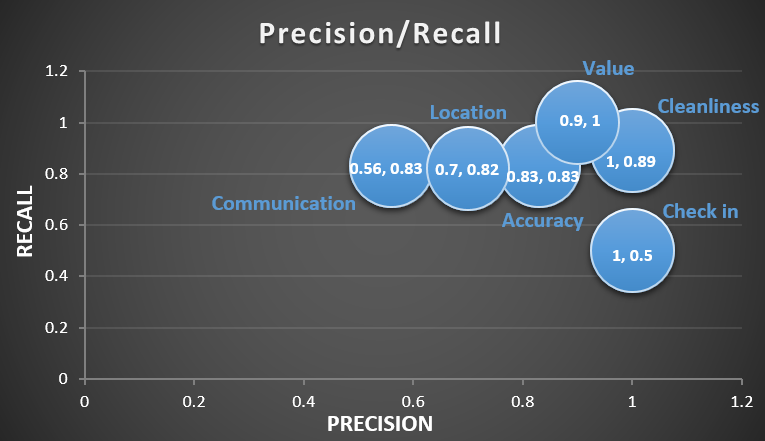
\includegraphics{precision_recall_1}
	\caption{Precision/Recall matrix for feature identification}
	\label{fig:matrix}
\end{figure}